\documentclass[oneside,final,14pt,a4paper]{extreport}

% # set the compiler XeLatex to use fontspec package
\usepackage{fontspec}
\usepackage{tempora}
\usepackage{newtxmath}

%\setmainfont{Times New Roman}

\usepackage{vmargin}
\setpapersize{A4}
\setmarginsrb{2.5cm}{2.2cm}{2.2cm}{2.2cm}{0pt}{10mm}{0pt}{13mm}
\usepackage{setspace}
\sloppy
\setstretch{1.5}
\usepackage{indentfirst}
\parindent=1.25cm

%%%%% ADDED TO SUPPORT TT BOLD FACES %%%%
\DeclareFontShape{OT1}{cmtt}{bx}{n}{<5><6><7><8><9><10><10.95><12><14.4><17.28><20.74><24.88>cmttb10}{}
% \renewcommand{\ttdefault}{Computer Modern}
%%%%% END %%%%%%%%%%%%%%%%%%%%%%%%%%%%%%%
\usepackage{atbegshi,picture}
\usepackage[T1]{fontenc}
\usepackage[utf8]{inputenc}
\AtBeginShipout{\AtBeginShipoutUpperLeft{%
  \put(\dimexpr\paperwidth-1cm\relax,-1.5cm){\makebox[0pt][r]{
\includegraphics[width=3cm]{figs/inno}}}%
}}


\usepackage[english]{babel}
\usepackage[backend=biber,style=ieee,autocite=inline]{biblatex}
\bibliography{ref.bib}
\bibliography{80211.bib}
\bibliography{ProprietaryTechnologies.bib}
\bibliography{RRM.bib}
\DefineBibliographyStrings{english}{%
  bibliography = {References},}
\usepackage{blindtext}


\usepackage{pdfpages}
\newenvironment{bottompar}{\par\vspace*{\fill}}{\clearpage}
\usepackage{amsmath,amsfonts}
\DeclareMathOperator*{\argmin}{argmin}
\DeclareMathOperator*{\argmax}{argmax}
\usepackage{url}

\let\openbox\relax
\usepackage{amsthm}
\newtheorem{theorem}{Theorem}
\newtheorem{corollary}{Corollary}
\newtheorem{lemma}{Lemma}
\newtheorem{proposition}{Proposition}
\theoremstyle{definition}
\newtheorem{definition}{Definition}
\theoremstyle{remark}
\newtheorem*{remark}{Remark}
\theoremstyle{remark}
\newtheorem*{example}{Example}

\usepackage{ifluatex}
\ifluatex
  \usepackage{pdftexcmds}
  \makeatletter
  \let\pdfstrcmp\pdf@strcmp
  \let\pdffilemoddate\pdf@filemoddate
  \makeatother
\fi
\usepackage{svg}

\newcommand{\card}[1]{\lvert{#1}\rvert}


\usepackage{titlesec}
\usepackage{float}
\usepackage{graphicx}
\graphicspath{{figs/}} %path to images
\usepackage{array}
\usepackage{multirow,array}
\usepackage{caption}
\usepackage{svg}
\usepackage{subcaption}
\usepackage{hyperref}
\usepackage{paralist}
\usepackage{listings}
\usepackage{zed-csp}
\usepackage{fancyhdr}
\usepackage{csquotes}
\usepackage{color}
\usepackage{xcolor}


\usepackage{chngcntr}
\usepackage{upgreek}
\usepackage{tabularx}
\usepackage{bm}
\usepackage{hyperref}
\usepackage{setspace}
\usepackage{booktabs}
\usepackage{multirow}
\usepackage{longtable}
\usepackage[font=singlespacing, labelfont=bf]{caption}
\counterwithout{table}{chapter}
\renewcommand{\thetable}{\Roman{table}}
%Hints
\newcommand\pic[1]{(Fig. \ref{#1})} %Ref on figure
\newcommand\tab[1]{(Tab. \ref{#1})} %Ref on table

\setlength{\headheight}{32.0976pt}
\usepackage{enumitem}
\newlist{inlinelist}{enumerate*}{1}
\setlist*[inlinelist,1]{%
  label=(\arabic*),
}

\setcounter{secnumdepth}{4}
\captionsetup[table]{labelfont={normalfont}, name={TABLE}, labelsep={newline}}
\counterwithout{table}{chapter}
\renewcommand{\thetable}{\Roman{table}}
\setlength{\parindent}{2em} 
\DeclareCaptionLabelSeparator{figSep}{.\quad}
\captionsetup[figure]{labelfont={normalfont}, name={Fig.}, labelsep=period}
\counterwithout{figure}{chapter}

\titleformat{\section}[hang]{\fontsize{20}{24}\selectfont\filcenter}{\Roman{section}}{1em}{}
\titleformat{\subsection}[hang]{\itshape}{\Alph{subsection}.}{1em}{}[]
\titleformat{\subsubsection}[runin]{\itshape}{\arabic{subsubsection})}{1em}{}[$:$]
\titlespacing{\subsubsection}{1em}{1em}{1em}
\titleformat{\paragraph}[runin]{\itshape}{\alph{paragraph})}{1em}{}[$:$\quad]
\titlespacing{\paragraph}{2em}{1em}{1em}

\pagestyle{fancyplain}
\usepackage{afterpage}

% remember section title
\renewcommand{\chaptermark}[1]%
	{\markboth{\chaptername~\thechapter~--~#1}{}}

% subsection number and title
\renewcommand{\sectionmark}[1]%
	{\markright{\thesection\ #1}}

\rhead[\fancyplain{}{\bf\leftmark}]%
      {\fancyplain{}{\bf\thepage}}
\lhead[\fancyplain{}{\bf\thepage}]%
      {\fancyplain{}{\bf\rightmark}}
\cfoot{} %bfseries


\newcommand{\dedication}[1]
   {\thispagestyle{empty}

   \begin{flushleft}\raggedleft #1\end{flushleft}
}

% \usepackage{algorithm}
% \usepackage{algorithmicx}
% \usepackage{algpseudocode}
\usepackage[linesnumbered,ruled,vlined]{algorithm2e}
\begin{document}

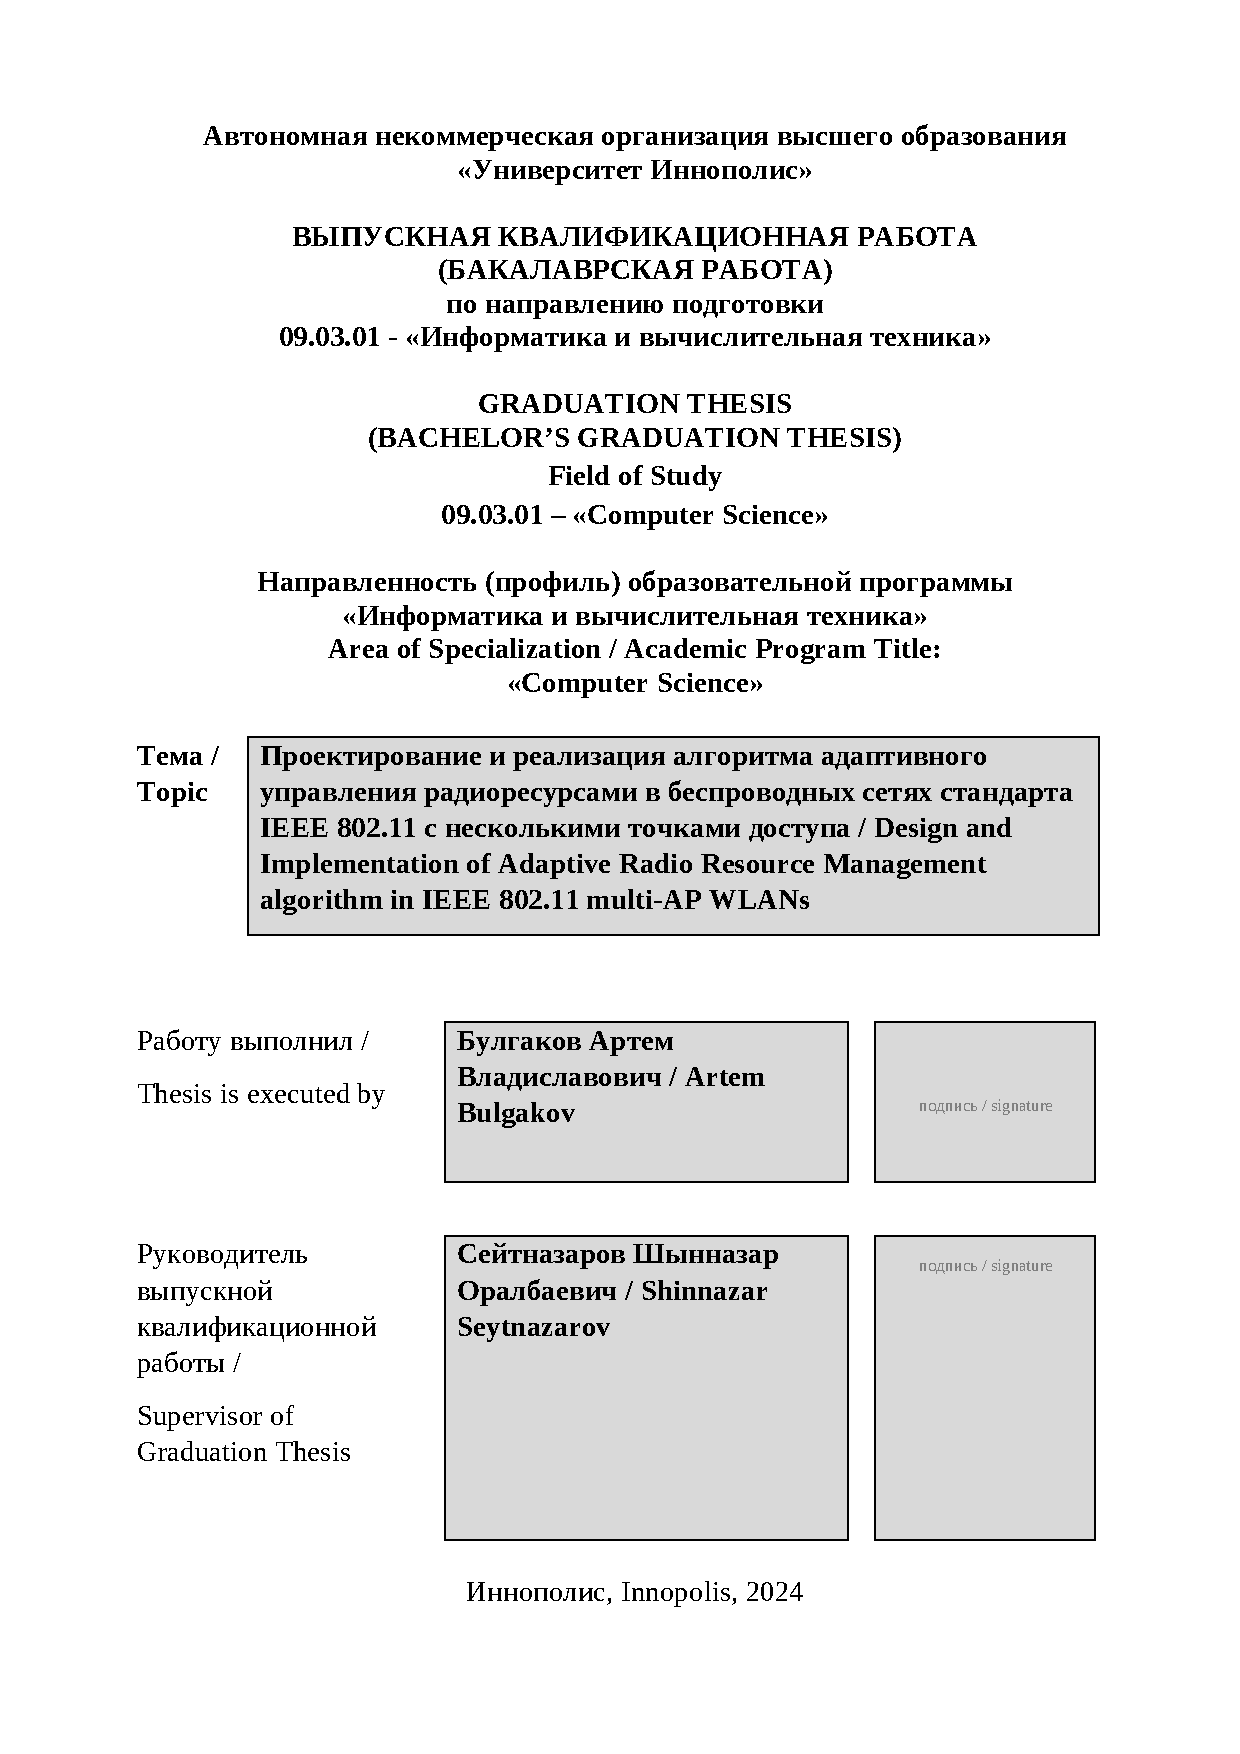
\includepdf[offset=70 -60]{title.pdf}
\tableofcontents
\listoftables
\listoffigures
\listofalgorithms
\renewcommand{\figureautorefname}{Fig.}
\renewcommand{\chapterautorefname}{Chapter}
\renewcommand{\sectionautorefname}{Section}


\newpage
\begin{abstract}
As IEEE 802.11 Wireless Local Area Networks (WLANs), also known as Wi-Fi, become ubiquitous, the increasing density of WLAN deployments leads to congestion of frequency bands and performance degradation due to interference. Thus, Radio Resource Management (RRM) algorithms for mitigating these problems are in demand, especially for dense WLAN deployments.

Although there are several commercial RRM solutions, their implementation details remain undisclosed. Moreover, such solutions are incompatible between devices produced by different vendors. At the same time, most of the previous studies have considerable obstacles for production usage.

In this study, I perform a theoretical analysis of \textit{RRMGreedy}, a centralized RRM algorithm used by a major Russian telecommunications vendor. I show that \textit{RRMGreedy} possess a number of flaws and tends to yield suboptimal results.
After identifying flaws of the algorithm, I propose several improvements for \textit{RRMGreedy}. The updated version of the algorithm is referred to as \textit{RRMGreedy++}. This algorithm adjusts frequency channel and transmission power parameters of access points based on physical-layer metrics, and uses WLAN Controller (WLC) as a central entity to gather data and perform computations.

Furthermore, this study develops a novel framework for the ns-3 network simulator that is used to implement \textit{RRMGreedy++} together with other RRM algorithms.
The simulation results demonstrate that \textit{RRMGreedy++} achieves up to a 12\% higher throughput on 2.4 GHz IEEE 802.11n networks and is capable of improving signal quality, measured in SNR (Signal-to-Noise Ratio) by 10\%.

% The RRMv2 algorithm employs unsophisticated metrics that can be obtained from the majority of OpenWRT-based Wi-Fi access points available on the market, demonstrating that the algorithm is production-ready and can be easily integrated into existing enterprise WLAN infrastructures.
\end{abstract}
\afterpage{%
  \pagenumbering{arabic}
  \setcounter{page}{1}
}
% \setcounter{page}{8} % set manually an actual number from which introduction starts
\chapter{Introduction}
\label{chap:intro}
\chaptermark{}

% indicate the importance of your topic
\section{Importance of the topic}

Nowadays, wireless local area networks (WLAN) implementing IEEE 802.11 standards, commonly known under "Wi-Fi" brand, become an increasingly popular solution for last-mile internet access with a diverse population of users, starting from home Wi-Fi routers up to large campus- and city-scale WLANs with coverage areas reaching several square kilometers.
As a result, the density of Wi-Fi network increases, so the frequency band allocated for 802.11 networks becomes more congested, which leads to interference and signal cancellation between different WLANs, resulting in network performance degradation.
Moreover, other appliances operating on frequencies that overlap with Wi-Fi band, undermining the performance of WLANs.
To meet current bandwidth and latency expectations of modern network applications, such as video streaming, cloud computing, and video conferencing, the wireless network must be able to provide sufficient capacity to all clients. In this light, proper radio resource management becomes crucial for operating wireless networks.

The problem of managing radio resources is studied extensively in the context of \textbf{cellular networks}, which are characterized by extensive frequencies reuse, large number of clients and large coverage areas spanning multiple kilometers, so the proper spectrum management is vital for operation of cells. This problem breaks down to the following: given a set of access points (or base stations in cellular terminology) $\boldsymbol{B}$, which can communicate over a set of channels $\boldsymbol{C}$, with a maximum transmit power of $P_{max}$, establish a radio link between a client device and an access point by assigning it a triplet $(b, c, p)$, where $b \in \boldsymbol{B}$, $c \in \boldsymbol{C}$, $p \leq P_{max}$.
Essentially, RRM algorithms aim to provide such assignments that maximize the overall network performance.
% indicate a lack or a gap in existing literature, possible limitations of the existing approaches
\section{Limitations of existing approaches}
A growing demand for Radio Resource Management (RRM) solutions, especially for large enterprise-grade multi-AP WLAN deployments, has led to the development of multiple commercial solutions, such as Cisco Radio Resource Management (RRM) \cite{ciscoRadioResourceManagement}, Aruba Adaptive Radio Management (ARM) \cite{UnderstandingARM}, and others. However, existing solutions offered by major vendors are proprietary, so their source code, used algorithms, and details of operation are not disclosed.
In the same time, most studies on RRM have only focused on cellular networks, while RRM in 802.11 networks received much less attention. Many existing works on RRM in 802.11 networks have applicability problems, since real-world hardware poses constraints on what metrics can be retrieved from the wireless interface and which physical and link-level parameters can be adjusted.

\section{Research gap}
Therefore, I can identify a research gap: the need for an open-source RRM (Radio Resource Management) algorithm that matches the performance of proprietary solutions and is feasible for real-world WLAN deployments.

This study aims to fill this gap by proposing a new RRM algorithm that, unlike existing market solutions, is publicly available, and at least as effective, while being practical and applicable to real-world WLAN deployments.

% indicate the contribution of your thesis project, establish its significance
\section{Contribution and significance of the study}
By analyzing theoretical works on 802.11 RRM, we come up with suitable optimization approach that combines both Adaptive Channel Selection (ACS) and Transmit Power Control (TPC) techniques to improve RF spectrum situation EM compatibility and channel reuse, which in turn leads to improved capacity of a wireless network.

Our RRM approach is encompassed within the centralized architecture, introduced by Cisco as Unified Wireless Network (UWN) \cite{CiscoUnifiedWirelessa}, a highly centralized wired-wireless architecture controlled by a Wireless LAN Controller (WLC). This approach allows for a more efficient spectrum management, as the WLC can collect data from all access points and make decisions based on the global view of the network, which is not possible in a distributed architecture, where each access point makes decisions independently.

% Outline of paper structure

The rest of this Thesis is structured as follows: Chapter \ref{chap:lr} reviews existing academic research on managing radio resources and publicly available information about proprietary RRM solutions; in Chapter 3, we formulate the mathematical model of transmission in a wireless network, review the existing RRM algorithm at Wimark Systems, identify its limitations and derive a new algorithm; in Chapter 4, we describe implementation details for the algorithm in NS-3 simulator and Wimark products; in Chapter 5, we evaluate the performance of our algorithm; Chapter 6 contains the results and discussion.


\chapter{Literature Review}
\label{chap:lr}
\chaptermark{}
The purpose of this chapter is to explore existing approaches on Radio Resource Management (RRM) in IEEE 802.11 networks, including surveying what is proposed as a part of the 802.11 standard itself, what research has been done and what is offered by existing commercial solutions. This chapter is organized as follows:
\begin{itemize}
    \item Section \ref{chap:lr:sec:80211_overview} briefly review the fundamentals of Radio Frequency (RF) communications, and IEEE 802.11 standard for wireless LAN;
    \item Section \ref{chap:lr:sec:rrm_80211} provides an overview how radio resource management is facilitated within the IEEE 802.11 standard;
    \item Section \ref{chap:lr:sec:prev_works} provides a synthesis on previous research in radio resource management;
    \item Section \ref{chap:lr:sec:prop_rrm} provides an overview of proprietary RRM solutions from major vendors;
    \item Section \ref{chap:lr:sec:conclusion} summarizes the chapter.
\end{itemize}
Table \ref{appx:defs_table} contains the list of definitions used in this chapter.

\section{Overview of IEEE 802.11 standard}
\label{chap:lr:sec:80211_overview}

Throughout this Thesis, I refer to domain-specific terms, whose definitions are given in Table \ref{defs_table}. Below in this chapter, I briefly review IEEE 802.11 standard and highlight the aspects most relevant for this study.


\subsection{Transmission medium}

The primary medium for communications in IEEE 802.11 are electromagnetic (EM) radio-frequency (RF) waves operating within the microwave range \cite{colemanCWNACertifiedWireless2021}.

\subsection{Frequency band}
Main frequency bands are: 2.4 GHz band introduced by 802.11b, 5 GHz band introduced by 802.11a and 6 GHz, introduced by 802.11ax. This study focuses on first two bands as used the most frequently. Below I describe those bands in more details.

Most of the 802.11 amendments, including b,g,n, and partially ax, operate at unlicensed 2.4 GHz ISM (Industrial, Scientific, Medical) RF band \cite{tanenbaumComputerNetworks2020, colemanCWNACertifiedWireless2021}. Using an unlicensed frequency band, however, introduces multiple challenges: the radio spectrum becomes congested with non-802.11 sources, such as microwave ovens, Bluetooth Personal Area Networks (PAN), cordless phones etc. \cite{tanenbaumComputerNetworks2020, colemanCWNACertifiedWireless2021}. Moreover, 2.4 GHz signals can propagate through solid obstructions like walls, doors, and windows better than signals operating on higher-frequency ones \cite{colemanCWNACertifiedWireless2021}. This property can provide better coverage and signal quality for clients, although can cause interference for neighboring WLANs, which will in turn lead to degradation of signal quality.

The 2.4 GHz ISM band is split into 14 channels. Depending on local regulations, number of possible channels can vary, but in general channels 1-11 are available at every region. Assuming 20 MHz channel width, each channel is characterized by its \textit{center frequency}, $\pm$ 10 MHz, with 5 MHz width between two adjacent centers, i.e, the channels \textit{overlap}. Channel 1 has central frequency 2.412 GHz, Channel 14 — 2.484 GHz. Thus, for channels to be non-overlapping, they must have at least 5 channels or 25 MHz in between. Such non-overlapping channels are 1, 6, 11, with central frequencies 2.412, 2.437, and 2.462 MHz, respectively.

The 5 GHz U-NII (Unlicensed National Information Infrastructure) series of bands is used by 802.11a/802.11ac/802.11ax amendments. Unlike the 2.4 GHz band, channels do not overlap. On the end of each band \textit{guard band} as an additional measure to avoid interference. Combined, bands U-NII-1, U-NII-1, U-NII-2A, U-NII-2C, U-NII-3 provide twenty-five 20 MHz or twelve 40 MHz non-overlapping channels \cite{colemanCWNACertifiedWireless2021}. However, some channels may not be available in different regions, since this band can also be used by military and weather radars. The first channel from U-NII-1 band has number 36.


\subsection{Signal quality and its metrics}

Thus, the presence of physical obstructions, background noise and interference from other access points urges us to explore possible measurements and metrics for a wireless signal quality. Below, I briefly describe the most widely used quantities:

A measure widely used in RF engineering and employed by Wi-Fi vendors is \textbf{Signal-to-Noise Ratio (SNR)}, which is defined as a ratio between the received signal power and the power of background noise:
\begin{equation}
    \label{formula:snr}
    SNR = \frac{P_{signal}}{P_{noise}}
\end{equation}
    Since SNR is essentially a difference in power, which is measured in Watts, in practice it is measured in a relative unit on a logarithmic scale called \textbf{decibel (dB)} [1,2]:

\begin{equation}
    \label{formula:snr_db}
    {SNR}_{dB} = 10\log_{10}\frac{P_{signal}}{P_{noise}}
\end{equation}

In recent years, \textbf{Signal-to-Interference-Plus-Noise ratio (SINR)} measurement have become a more widespread measurement of wireless networks\' signal quality. Similarly, it is defined as:

\begin{equation}
    \label{formula:sinr}
    SINR = \frac{P_{signal}}{P_{noise} + P_{interf}}
\end{equation}

    where $P_{signal}$ is the power of the signal of interest, and $P_{interf}$ is the power of interfering signals.
    By considering interference from other 802.11 devices, which is typically a dynamic quantity that changes rapidly over time unlike background noise, SINR describes EM spectrum situation more accurately.

Received Signal Strength Indicator (RSSI) relative measure of signal strength in range from 0 to 255, where 0 is the weakest signal a receiver is able to sense. The exact correspondence between RSSI and received signal power is implementation-specific and is left on behalf of hardware manufacturers \cite{colemanCWNACertifiedWireless2021}.

\subsection{Radio Resource Management}
\label{chap:intro:sec:rrm}
The scarcity of available frequency bands in the time of growing demand for wireless connectivity has led to the development of methods called \textit{spectrum management} or \textit{radio resource management (RRM)}. Most of research on RRM is focused on cellular networks, where coverage area of base stations spans across multiple kilometers, and the number of clients for one station can reach several thousands, so proper spectrum management is vital for operation of cells. However, from the physical layer perspective, the radio situation in 802.11 networks is similar. As described in \cite{zanderRadioResourceManagement1997}, given a wireless network with a set of access points $\boldsymbol{B}$, which can communicate over a set of channels $\boldsymbol{C}$, with a maximum transmit power of $P_{max}$, establishing a radio link between a client device and an access point requires from the wireless infrastructure to assign:
\begin{enumerate}
    \item An access point $b \in \boldsymbol{B}$;
    \item A frequency channel $c \in \boldsymbol{C}$;
    \item A transmission power level $ p \leq P_{max}$.
\end{enumerate}
Obviously, channel and transmission power are \textit{global} for a given access point in a sense that all its other clients will have to adjust their parameters correspondingly: switch the operating channel and deal with the new received signal strength from their AP.
In Wi-Fi, the first requirement is usually managed by the client itself: user chooses SSID they wish to use, and in case if multiple APs serve the same SSID, a client device associates with AP having the strongest signal available. Later, a client can switch to another access point within the same extended service set via \textit{roaming} methods, such as \textit{Fast Basic Service Set (BSS) Transition} defined in 802.11r \cite{80211r2008IEEE}. The roaming decision is ultimately made by a client device, which sends a reassociation request to start the roaming process \cite{colemanCWNACertifiedWireless2021}. The access point, however, can force a client to find another access point by sending a deauthentication frame, or moving to another channel without notifying.
The second and third requirements are a part of current AP configuration and a subject to change. A client discovers current operating channel of APs by tuning on each available channel in a succession, while transmission power only can be estimated by measuring received signal strength.
Thus, \textbf{the goal of a radio resource allocation algorithm is to optimize spectrum usage within a WLAN via assigning an operating channel and a transmission power level to each access point in a way that maximizes the overall network performance.}

As it will be shown in Section \ref{chap:lr:sec:rrm_80211}, the 802.11 standard does not provide any algorithms for channel and transmission power assignment, however, some amendments introduce methods for measurement, signaling and radio adjustment that can be used for RRM purposes.

Note that related researches and commercial solutions introduce many similar terms for the same procedure of channel change that can use different algorithms and slightly vary according to specifics of their application: \textit{Frequency Selection}, \textit{Frequency Planning}, \textit{Channel Selection}, \textit{Channel Planning}, \textit{Channel Assignment}, etc. Adjustment of transmission power is usually
In this study, we use those terms interchangeably.

\section {Radio Resource Management in IEEE 802.11}
\label{chap:lr:sec:rrm_80211}
As described in Section \ref{chap:intro:sec:rrm}, a radio resource management algorithm aims to optimize network capacity through optimizing spectrum usage by adjusting two parameters: frequency and transmission power of each access point. The very need for an RRM algorithm comes from situation called \textit{Overlapping Basic Service Sets} in the IEEE 802.11 standard, when there are two basic service sets operating on the same channel within reach of each other. This situation leads to co-channel interference, which degrades network performance. In this section, I provide an overview of methods and techniques provided by IEEE 802.11 standard that can assist in radio resource management.


\subsection {IEEE 802.11h}
\label{chap:lr:sec:80211h}
To comply with legal requirements on transmissions in 5 GHz, 802.11h-2003 \cite{ieee80211h} amendment (\textit{Spectrum and Transmit Power Management Extensions}) was introduced. Since the goal of this amendment is to prevent legacy 802.11a 5GHz APs from interference with radars, 802.11h is not oriented for optimizing capacity of a wireless network. However, 802.11h introduces \cite{konsgenSpectrumManagementAlgorithms2010} spectrum management methods, namely, \textit{Dynamic Frequency Selection (DFS)}, facilitating automatic change of AP's operating frequency, and \textit{Transmit Power Control (TPC)}, adjusting the power of AP's transmitter.
Those methods, however, do not implement RRM in the sense of optimizing network capacity, but rather are aimed at preventing interference with radars operating on the 5 GHz band. 802.11h describes procedures for: quieting the channel to detect presence of a radar, switching to another channel if a radar detecting, advertising the channel switch to client stations (STAs). However, the description of a radar detection procuedre is beyond the scope of 802.11 standard \cite{ieee80211h}.
However, the frame types and measurement reporting mechanisms introduced in 802.11h can be considered as a foundation for further research on RRM algorithms.


% \subsubsection{Transmit Power Control}

\subsection {IEEE 802.11k}
\label{chap:lr:sec:80211k}
The amendment 802.11k-2008 \cite{ieee80211k} (\textit{Radio Resource Measurement}, not to be confused with \textit{Radio Resource Management}) improves the performance of roaming. Roaming is a process of station moving from one access point to another \cite{colemanCWNACertifiedWireless2021}. The amendment 802.11k improves roaming by allowing stations to request from access points various reports, such as \textit{neighbor reports} for discovering possible access points that STA can roam to, \textit{link measurements} to estimate how well AP can hear the station etc. This allows stations to reduce power consumption, speed up roaming and decrease power consumption and airtime usage spent on sending probe requests to each channel when trying to find another AP to roam.
However, this amendment is also not aimed at optimizing network capacity, but rather at improving roaming performance.

\subsection {IEEE 802.11ax}
\label{chap:lr:sec:80211ax}

The amendment 802.11ax \cite{80211ax} (\textit{High Efficiency WLAN}) introduces means to address OBSS problem. The amendment introduces \textit{Basic Service Set (BSS) Coloring}, a method to distinguish between different BSSs operating on the same channel. It works as following: each BSS is assigned with \textit{color}, a 6-bit value spanning from 1 to 63, that resides in the PHY header. Devices belonging to the same BSS check this color when demodulating transmissions (i.e., check if this frame is an \textit{intra-BSS}). If it contains the wrong color (\textit{inter-BSS} frame), further demodulation is not performed, thus saving processing time \cite{CiscoCatalyst9800}.
If an intra-BSS frame is found to use the same color, AP switches to another color.
One can see that such solution completely relies on CSMA/CA media access control (MAC) mechanism and is not able to address hidden terminal problem. That is, if AP providing overlapping BSS is a hidden terminal, the signal will be disrupted near the destination, so the receiving station will not be able to demodulate the signal to inspect the color tag.
Thus, this technique does not solve the problem of co-channel interference and does not provide channel planning, so this cannot be considered as a complete RRM solution.



\section {Previous Works}
\label{chap:lr:sec:prev_works}
Interference from other Access Points poses a serious obstacle \cite{suiHowBadAre2015} for delivering acceptable quality of service in large 802.11 WLAN deployments. Although the 802.11 carrier-sense MAC protocol is designed to be resilient to interference, interference reduces the available airtime and causes loss of frames already sent. Thus, network capacity and performance tend to degrade drastically \cite{levantiCAPWAPCompliantSolutionRadio2007}. For interference between cells within a single WLAN, such problem in principle can be solved by proper \cite{site surveying}, i.e., planning of geographical placement of cells. However, another and the major source of interference are \text{rogue access points} (RAPs), which are operated by third parties and in general are not under control of WLAN administrators. According to \cite{suiHowBadAre2015}, interference from rogue APs can introduce up to 50\% delays in a WLAN. Moreover, the prevalent amount (more than 70\%) of rogue APs are stationary \cite{suiHowBadAre2015}, so their radio presence can be considered as a constant factor in the WLAN. Note that \textit{rogue} does not imply that those APs are malicious or posing threats other than congesting channels and occuping airtime as a result of their legitimate operation.
In this light, attempts to improve spectrum management via channel assignment and transmit power control adjustment algorithms encompass research on Radio Resource Management algorithms. As shown in Section \ref{chap:lr:sec:rrm_80211}, the IEEE 802.11 standard provides a limited set of tools for radio resource managemens, leaving assignment algorithms and policies on behalf of WLAN equipment vendors. As reported in \cite{suiHowBadAre2015}, Cisco's RRM software, shipped with Cisco Aironet APs and Cisco WLAN Controller, was able to improve network performance using Dynamic Channel Selection (DFS) and Transmit Power Control (TPC)  so that carrier sense interference was responsible for only 5\% of network delays. RRM solutions from Cisco and other vendors will be surveyed in Section \ref{chap:lr:sec:prop_rrm}. However, since those technologies are proprietary, their implementation details are not disclosed, so they cannot be properly evaluated in an independent research or adopted by third-party vendors. Moreover, such solutions lack interoperability, so it is difficult to use them with networking products from other vendors, which is a major obstacle for large-scale WLAN deployments and leads to vendor lock-in situations. Thus, research on radio resource management algorithms is important for the industry.

\subsection {Radio Resource Management Approaches}
\label{chap:lr:sec:rrm_approaches}
Since RRM is a broad topic which does not imply a single methodology, approach, or even a definition, classification of RRM algorithms is a challenging task. Most of the papers with the "Radio Resource Management" keyword are focused on problems of cellular networks, such as LTE or 5G. At the same time, the problem formalization, some optimization objective and algorithms can also be used for research in 802.11 networks, but band usage, client management, deployment and operation specifics make most of the proposals inapplicable for 802.11 networks.
To the best of my knowledge, no comprehensive survey on RRM in 802.11 WLAN exist. I will refer to \cite{bouhafsPerFlowRadioResource2020}, which provides detailed overview of previous research, and \cite{leeDeepLearningAidedChannel2023}, describing state-of-the-art on RRM.
In \cite{bouhafsPerFlowRadioResource2020}, authors classify RRM algorithms into three categories:
\begin{itemize}
    \item \textit{per-cell} approaches seek to optimize the RF situation within the AP's cell coverage. This means that adjustments of radio parameters applied on a cell scale and will be in effect for all stations within the cell. Such classification can be further divided into:
    \begin{itemize}
        \item \textit{localized (uncoordinated) per-cell}, where each AP performs RRM decisions independently;
        \item \textit{centralized per-cell}, where a central entity, such as WLAN Controller, performs RRM decisions for all APs within a WLAN. Some authors refer to this approach as \textit{super-cell} approach \cite{levantiCAPWAPCompliantSolutionRadio2007}; \item \textit{coordinated per-cell}, employing cooperation between APs for making coordinated RRM decisions.  \end{itemize} \item \textit{per-link} approaches, which optimize the transmission power for a given station; \item \textit{per-flow} approaches, which employ frequency and AP Tx power adjusting to optimize the QoS to the granularity of a given traffic flow within a station, for example, to the flow of a VoIP application.
\end{itemize}

In fact, a simple localized per-cell RRM is already widely implemented: almost every home Wi-Fi router has the option to select channel automatically. Typically, in this case access point surveys each channel, makes an estimation how congested it is, then switches to the least congested one. This technique is called \textit{least-congested channel scan}, or \textit{least-congested channel search} (LCCS), and the original design uses the number of associated clients as estimation of channel congestion \cite{achantaMethodApparatusLeast2006}.
As analyzed in \cite{aruneshmishraWeightedColoringBased2005}, LCCS has several limitations:
\begin{enumerate}
    \item LCCS is unable to accurately identify interference scenarios where clients connected to different Access Points (APs) interfere with each other without the APs themselves causing interference. This issue is particularly prevalent in real-world setups where APs are strategically placed to ensure wide coverage while overlapping minimally to avoid coverage gaps;
    \item LCCS also falls short in optimizing channel reuse based on the distribution of clients. It fails to account for the interference experienced by clients, thus missing the opportunity for channel reuse strategies based on client locations and densities.
\end{enumerate}

In general, uncoordinated decision-making like LCCS tends to yield suboptimal results. Consider an extreme case, where a number of APs can sense that channel $C_i$ is not congested and make a decision to switch to that channel. As a result, $C_i$ becomes congested, so APs will seek to switch to another channel $C_j$, where the problem will reoccur. This situation suggests that using a coordinated RRM policy between APs can improve overall WLAN capacity and thus achieve a global optimum.

Research on Transmit Power Control (TPC) methods, which adjust transmission power $P_{Tx}$ to maintain an acceptable Signal-to-Noise-plus-Interference Ratio (SINR), shows potential for enhancing bandwidth. However, criticisms regarding these studies' simplified models, unrealistic experimental setups, and statistically uncertain outcomes suggest the need for further investigation \cite{michalskiSimplePerformanceboostingAlgorithm2016,kazminIspolzovanieNeyronnyhSetey2021}. The effect of IEEE 802.11 roaming on TPC is underexplored, especially in scenarios where APs are part of the same extended service set (ESS), which is more common in enterprise WLANs.

As shown in \cite{ramachandranSymphonySynchronousTwophase2008}, per-link TPC considerably improves WLAN performance, achieves more spatial reuse, increases throughput, and able to avoid channel access asymmetry and receiver-side interference (also known as hidden-node problem). However, such approach has certain hardware requirements, namely, \textit{per-packet transmit power control}, a feature available only for a small selection of 802.11 chipsets.
In turn, implementing per-flow RRM in standard 802.11 networks requires an advanced framework for identifying specific traffic flows and assessing their Quality of Service (QoS) demands \cite{bouhafsPerFlowRadioResource2020}. Therefore, this thesis will concentrate on solutions that are more practical and applicable to the hardware and software currently available on the market.

\subsection{Mathematical Models for Radio Resource Management}
\label{chap:lr:sec:math_models}

Building on the definition of the Radio Resource Management (RRM) problem introduced in \ref{chap:intro}, we consider a network composed of a set of base stations (access points) denoted as $\boldsymbol{B}$, capable of operating over a collection of channels $\boldsymbol{C}$, each with a maximum transmission power limit $P_{max}$. The core objective of RRM is to establish a radio link between a client device and an access point by assigning a triplet $(b, c, p)$, where $b \in \boldsymbol{B}$ signifies the base station, $c \in \boldsymbol{C}$ the channel, and $p \leq P_{max}$ the transmission power, so that network capacity is maximized.

The RRM problem, thus, decomposes into three crucial tasks:
\begin{itemize}
\item \textit{Client Assignment} --- allocating a base station (access point) to a client;
\item \textit{Adaptive Channel Selection} --- determining the optimal frequency (channel) for client communication;
\item \textit{Transmit Power Control} --- setting the appropriate transmission power for client communication.
\end{itemize}

Client Assignment is typically handled by the 802.11 client through roaming decisions, with amendments like 802.11k/r/v designed to enhance and expedite the process of switching to an access point that offers superior service quality. This aspect, therefore, lies beyond the scope of this study.

Channel allocation and transmit power selection, though extensively studied, are often addressed as separate entities in the literature. Combining these factors introduces complexity, as their objectives can conflict. For example, if the objective is to minimize interference, it can be achieved with minimizing the transmission power. However, such outcome probably does not satisfy coverage and quality of service requirements. On the other hand, considering channel and transmit power together can also be troublesome, since change in one variable would change the overall RF situation, and the algorithm would not converge.

Another aspect is choice of metrics. Although the most intuitive and desired metrics are high-level ones like network throughput and capacity, actual values of such metrics cannot be used at the time of RRM computations: a significant time of monitoring is required to estimate how throughput changed, so only past records can be used. Another, simpler approach, followed by many works, is to assume that network throughput or capacity is a function of one or more physical layer metrics, such as interference, Received Signal Strength Indicator (RSSI), Rx signal power etc. Indeed, low interference level and low power signal from other APs implies that less transmission errors tend to happen, and more frames can be transmitted with CSMA/CA MAC mechanism.
This reliance on physical layer metrics allows for more immediate adjustments in RF (Radio Frequency) configuration of a WLAN, ensuring the adaptability of the network to immediate environmental changes.
However, RRM adjustments in practice can lead to disruptions. Most client devices lack support for the Channel Switch Announcement feature from 802.11h, interpreting a channel switch as if the AP has become unavailable. Therefore, utilizing historical data becomes instrumental in making informed, albeit infrequent and periodic, RRM decisions.

Thus, channel and transmit power settings for each AP should yield optimal value of some given metric for the whole WLAN, such as: interference level, WLAN throughput, WLAN capacity, etc. Thus, most of the works consider RRM as an optimization problem, such as integer linear programming (ILP) \cite{leeOptimizationAPPlacement2002} \cite{rodriguesDesignCapacityPlanning2000} or binary quadratic programming (BQP) \cite{leeDeepLearningAidedChannel2023}.
Since both ILP and BQP are proven to be NP-hard problems, researchers propose heuristics to reduce search space \cite{levantiCAPWAPCompliantSolutionRadio2007}, or apply meta-heuristic methods such as genetic algorithms \cite{raschellaEvaluationChannelAssignment2019} or deep neural networks \cite{leeDeepLearningAidedChannel2023}. Other approaches, while not solving optimization problem explicitly, aim to keep some target metric, such as SINR (Signal-to-Interference-plus-Noise Ratio), within pre-defined acceptable boundaries \cite{michalskiSimplePerformanceboostingAlgorithm2016}.
In \cite{aruneshmishraWeightedColoringBased2005}, authors employ a graph model, where APs are represented as nodes and edges connect APs which can potentially interfere. Using such model, each node can be assigned a color representing its channel.

It is important to emphasize that in 802.11 WLANs, all clients connected to a specific Access Point (AP) utilize the same frequency and transmission power settings. Given the limited applicability of per-link (per-client) Transmit Power Control (TPC), as previously discussed, it is assumed that both frequency and transmission power are configured for the entire cell. This means that all clients of a given AP operate on the same frequency, and the AP maintains a consistent transmit power level for communication with all its clients.


\section {Proprietary RRM Solutions}
\label{chap:lr:sec:prop_rrm}
This section surveys proprietary RRM solutions offered by leading vendors in the enterprise WLAN market. I focus on Cisco, Juniper Networks, and Ruckus Networks, since they are the most popular vendors in enterprise WLAN market \cite{WiFiMarketSize}. To the best of my knowledge, peer-reviewed evaluations of those proprietary RRM efficiency are very limited and scarce, so one could only rely on the claims made by vendor themselves.

\subsection{Cisco}
Cisco's RRM strategy is integral to its Cisco Centralized Architecture, known as the Unified Wireless Network (UWN) \cite{CiscoUnifiedWirelessa}. In the UWN framework, a single or multiple Wireless LAN Controllers (WLCs) manage up to several thousand Access Points (APs). These WLCs act as the core of the WLAN architecture, enabling centralized control and the collection of telemetry from all APs within the network. A WLC can be either specialized hardware or a virtual machine hosted in the cloud \cite{arenaUnderstandingTroubleshootingCisco2022}.
Effectively, in UWN, access points can be thought of as Wi-Fi network interface cards for the WLC, providing minimal real-time functionality from 802.11 standard that cannot be carried out to WLC due to propagation and transmission delays.
This architectural model has become the de facto standard for large-scale enterprise WLANs and is employed by most major vendors in the industry.

Cisco offers several RRM solutions. First, CleanAir is a flagship technology from Cisco \cite{CiscoCleanAirTechnology2014} to optimize network performance, avoid jamming, and detect interference sources, including non-802.11 ones. Cisco states that it outperforms competitors through several features:

\begin{itemize}
    \item It utilizes specialized hardware for RF analytics. For instance, the Cisco Catalyst 9100 Series Access Points contain a scanning radio for background RF scanning. This functionality allows for continuous service provision to clients without disrupting the main AP radio transceivers. Additionally, the Cisco RF ASIC, a dedicated chip, enables advanced wireless network analytics and spectrum analysis unavailable to conventional Wi-Fi modules;
    \item Classifying and visualizing interference sources thanks to dedicated RF hardware;
    \item Comprehensive WLAN-wide radio resource management, supplying both real-time and historical data at varying levels of granularity;
    \item CleanAir is event-driven, that means it can adapt to changing RF environment and adjust radio parameters in a matter of few minutes, drastically reducing downtime.
\end{itemize}
However, CleanAir is only available for the higher-end models in the Cisco product line, posing limitations for its large-scale deployment. Furthermore, lack of compatible radio analytics hardware from other vendors and undisclosed implementation details restrict the utility of this technology for integration with non-Cisco equipment.
On the other hand, Cisco Catalyst product line of WLAN Controllers also provide "regular" RRM functionality that only requires regular Wi-Fi chipset and can be used with all Cisco APs \cite{ciscoRadioResourceManagement}. The trade-off for this convenience is access to less detailed information about the RF environment and the necessity for Access Points to temporarily switch off their current channel to conduct scanning. In this case, APs collect statistics on their current channel any time they are not transmitting data. Additionally, periodically APs scan other channels to gather statistics. \cite{arenaUnderstandingTroubleshootingCisco2022}. At that time, AP is not available to clients, so, scanning introduces latencies for the clients connected to the AP.

Cisco RRM employs a super-cell concept. In such scheme, a group of geographically close APs (forming an \textit{RF Group}) is managed by a designated WLAN Controller (\textit{RF Group Leader}).
A subgroup unit within an RF group is called \textit{RF Neighborhood}, and consists of AP that can hear each other at signal strength $\geq 80 \; dBm$ \cite{arenaUnderstandingTroubleshootingCisco2022}. Each AP is associated with two lists: RX neighbors, i.e., list of APs that given AP can hear, and TX neighbors, a list of APs that can hear given AP.
For each channel, Cisco RRM maintains a \textit{cost metric}, an estimation of channel goodness that is based on RSSI, co-channel interference, non-WiFi interference.


\subsection{Juniper Networks}
Juniper Networks offers Mist AI RRM technology to improve network performance. The notable features are \cite{junipernetworksUnderstandingRadioResource2023,RadioManagementTechnology}:
\begin{itemize}
    \item Automatic dual-band radio management --- if RRM system finds 2.4-GHz radio transmitter to be unused on a given AP, it disables the radio to free airspace for other access points;
    \item Juniper Mist APs incorporate the Predictive Analytics and Correlation Engine (PACE) "to monitor conditions and make out-of-band adjustments" \cite{RadioManagementTechnology};
    \item Telemetry is sent to the Juniper Mist Cloud, so that the cloud can periodically fine-tune APs based on historical data and usage statistics;
    \item Employing a Reinforcement Learning (RL) methodology for the strategic planning of channel selection and power settings across APs in a WLAN, aiming for optimal network performance \cite{junipernetworksUnderstandingRadioResource2023}.
\end{itemize}

\subsection{Ruckus Networks}
Ruckus Networks offers ChannelFly RRM technology, which provides automatic channel selection. ChannelFly estimates capacity of each channel by continuously monitoring the activity of each channel across the 2.4 and 5GHz bands. Based on this information, ChannelFly develops a statistical model to predict which channel will offer the highest capacity for clients, as detailed by \cite{RuckusChannelFlyFeature2023}. A key benefit of ChannelFly is its ability to avoid "dead time", defined as the period an AP spends scanning different channels, during which it cannot communicate with clients. This capability implies the inclusion of dedicated scanning radios in Ruckus APs, allowing continuous communication with clients while performing channel assessments.

Additionally, Ruckus offers a "smart adaptive antenna array" technology. This feature enhances the directionality of signals from Ruckus APs, focusing the transmission towards clients to improve the Signal-to-Noise Ratio (SNR).

\subsection{Aruba Networks}
The Adaptive Radio Management (ARM) technology by Aruba represents an earlier approach to Radio Resource Management (RRM), utilizing Adaptive Channel Selection and Transmit Power Control to enhance the RF environment in WLANs. ARM stands out for its algorithmic simplicity and the thoroughness of its documentation provided by Aruba, in contrast with other vendors \cite{ArubaOSUserGuide}.

Key features of ARM include \cite{ARMOverview}:
\begin{itemize}
\item \textbf{Application Awareness}: Addressing the "dead time" caused by APs during channel scanning, ARM throttles the frequency of background scans based on current traffic load, reducing scans under heavy traffic and resuming normal scanning rates when traffic diminishes \cite{UnderstandingARM}.
\item \textbf{Mode Awareness}: To mitigate interference in environments with densely installed APs, ARM can switch excessive APs to Air Monitor mode, where they continuously collect and send RRM telemetry to the controller.
\item \textbf{Band Steering}: Promotes the use 5 GHz band to clients, instead of more congested and higher-range 2.4 GHz band.
\item \textbf{802.11n HT Mode Support}: ARM can utilize a 40 MHz channel pair for 802.11n networks, selecting the best primary and secondary operating channels automatically.
\item \textbf{Noise and Error Monitoring}: Distinguishes between 802.11 and non-802.11 noise sources, improving network reliability.
\item \textbf{Spectrum Load Balancing}: Analyzes client distribution across neighboring APs to direct new connections to less burdened APs, though clients may reconnect to their original choice upon a subsequent attempt.
\item \textbf{Noise Interference Immunity}: Adjusts the receiver sensitivity threshold to ignore weak and non-802.11 signals, reducing unnecessary decoding efforts and improving network performance.
\end{itemize}

Reports from system administrators, though, suggest that RRM decisions in Aruba ARM are made by APs rather than controller. Among other user complains are unnecessary disabling of 2.4GHz radios, erroneous TPC leading to coverage holes \cite{TamingArubaARM2012}.

However, ARM is a legacy technology. Its successor, Aruba AirMatch, introduced in recent ArubaOS versions, is a more sophisticated RRM technology, which is based on AI and machine learning and is able to perform channel and power planning on a WLAN-wide scale, suggesting ARM was implemented in a per-cell way and AirMatch is a super-cell solution.

Notable AirMatch features:

\begin{itemize}
    \item Channel width adjustment based on device density - the more devices are connected to an AP, the narrower channel width is used to allow channel reuse and reduce interference;
    \item APs measure RF environment for 5 minutes every 30 minutes;
    \item Decisions based on a 24-hour period analytics unlike instant RF situation snapshots in ARM;
    \item Elimination of coverage holes based on TPC.
    \item Configurable thresholds in channel quality improvements to trigger channel and EIRP planning, default threshold is 15\%.
    \item ClientMatch technology that manages clients: performs load balancing between APs, encourages clients to switch to APs providing better signal strength and using higher bands (5 GHz or event 6 GHz in 802.11ax)
\end{itemize}

Similarly to ARM, Aruba provides more information about AirMatch operating logic than other vendors about their RRM solutions.

According to \cite{ArubaOSUserGuide}, AirMatch blacklists channel for channel selection if a radar was detected on it (in 5 GHz case) or in case if high noise level was detected on it (for all bands). In those cases, AirMatch will select channel with a manimum interference index.

It is not clear if AirMatch uses the same metrics as ARM, but only ARM metrics are described in the documentation.
To make RRM decisions, ARM uses two metrics:
\begin{itemize}
    \item \textbf{Coverage Index} - comprises two components, $x$ and $y$:
    \begin{itemize}
        \item $x$ is weighted calculation of Signal-to-Noise Ratio (SNR) for all APs on a given channel;
        \item $y$ is the weighted sum of the SNRs that neighboring APs within the group observe on the same channel.
    \end{itemize}
    \item \textbf{Interference Index} - measures co-channel and adjacent-channel interference, calculated as a sum of four quantities $a$, $b$, $c$, $d$:
    \begin{itemize}
        \item $c$ is the channel interference the AP neighbors see on the selected channel;
        \item $d$ is the interference the AP neighbors see on the adjacent channel.
    \end{itemize}
\end{itemize}
Additionally, Aruba APs collect several other metrics, including L2 metrics \cite{ArubaOSUserGuide}:

\begin{itemize}
    \item Number of Retry frames, measured in \%
    \item Number of Low-speed frames, measured in \%
    \item Number of Non-unicast frames, measured in \%
    \item Number of Fragmented frames, measured in \%
    \item Number of Bandwidth seen on the channel, measured in kbps
    \item Number of PHY errors seen on the channel measured in \%
    \item Number of MAC errors seen on the channel measured in \%
    \item Value of noise floor on the specified AP
\end{itemize}

Aruba documentation indicates that these metrics offer a "snapshot of the current RF health state" \cite{ARMMetrics}, suggesting they are informational tools for network administrators rather than being actively used in RRM decision-making.

% \section {Concerns and Requirements for an RRM algorithm}

\section {Conclusion}
\label{chap:lr:sec:conclusion}
Summarizing the insights from prior sections, I can conclude that the problem of radio resource management in 802.11 WLANs is still relevant, since the IEEE 802.11 standard provides only limited tools for RRM, while existing commercial solutions are proprietary and lack interoperability. Thus, there is a need for a novel RRM algorithm that can be implemented in existing enterprise WLAN infrastructure and improve overall network performance.

I find super-cell approach most fitting for a modern RRM algorithm that can be applied in real-world WLAN deployments. Super-cell algorithms, while being practical and having less obstacles in hardware and current device drivers compared to other approaches, still have the potential to vastly improve RF situation and, thus, WLAN performance.

Centralized management that is typically utilized in super-cell RRM is the standard approach when building modern WLANs, allowing to gather more information about RF environment and come up with more optimal allocations compared with local RRM decision-making.
Moreover, presence of WLC as centralized entity with orders of magnitude higher computation power and ability to collect and store statistics from all APs all over the WLAN in the long term releases the burden of RRM from Access Points and potentially improves the overall network efficiency.

Despite the promising capabilities of per-link and per-flow radio resource management approaches for optimizing wireless networks in a more fine-grained and application-aware manner, they have considerable limitations that currently prevent from implementing them in production wireless networking solutions.

As a summary of this survey, we can identify the research gap: the problem of radio resource management in 802.11 WLANs is still relevant, since IEEE 802.11 standard does not provide fully-fledged RRM, while existing commercial solutions are proprietary and lack interoperability. Thus, there is a need for an RRM algorithm addressing key issues, including:
\begin{itemize}
    \item Design for centralized management of enterprise WLAN, working as a part of Wireless LAN Controller;
    \item Applicability with current hardware and software, namely:
    \begin{itemize}
        \item Effortless integration with OpenWRT-based access points;
        \item Requires data like physical and link-layer statistics that can be obtained using only regular Linux Wi-Fi drivers like \texttt{nl80211}, and standard Linux networking tools;
    \end{itemize}
    \item Performing not worse than existing RRM algorithm \textit{RRMGreedy}, analyzed in Chapter \ref{sec:baseline};
    \item Able to combine both channel selection and transmit power adjustment to improve RF environment and network performance.
\end{itemize}

The following chapters will focus on analyzing the limitations of current algorithms and developing a new one.
\chapter{Methodology}
\label{chap:met}


\ldots

Referencing other chapters \ref{chap:lr}, \ref{chap:met}, \ref{chap:impl}, \ref{chap:eval} and \ref{chap:conclusion}
\begin{longtable}{c|c}
\caption[This is the title I want to appear in the List of Tables]{Simulation Parameters} \label{table:thisimulation_params} \\
\hline
A & B  \\
\hline
\endfirsthead
\multicolumn{2}{@{}l}{} \\
\hline
A & B \\
\hline
\endhead
\hline
 \textbf{Parameter} & \textbf{Value}\\
 \hline
 Number of vehicles & $|\mathcal{V}|$\\
 \hline
 Number of RSUs & $|\mathcal{U}|$\\
 \hline
 RSU coverage radius & 150 m\\
 \hline
 V2V communication radius & 30 m\\
 \hline
 Smart vehicle antenna height & 1.5 m\\
 \hline
 RSU antenna height & 25 m\\
 \hline
 Smart vehicle maximum speed & $v_{max}$ m/s\\
 \hline
 Smart vehicle minimum speed & $v_{min}$ m/s\\
 \hline
 Common smart vehicle cache capacities & $[50, 100, 150, 200, 250]$ mb\\
 \hline
 Common RSU cache capacities & $[5000,1000,1500,2000,2500]$ mb\\
 \hline
 Common backhaul rates & $[75, 100, 150]$ mb/s\\
 \hline
\end{longtable}

\begin{figure}[hbt]
\centering

\includegraphics[]{figs/inno.png}
\caption{One kernel at $x_s$ (\emph{dotted kernel}) or two kernels at
$x_i$ and $x_j$ (\textit{left and right}) lead to the same summed estimate
at $x_s$. This shows a figure consisting of different types of
lines. Elements of the figure described in the caption should be set in
italics, in parentheses, as shown in this sample caption.}
\label{fig:thiex}
\end{figure}


\ldots
\chapter{Implementation and evaluation}
\label{chap:impl}


This chapter is dedicated to implementing the RRMv2 algorithm described in Section \ref{chap:research:sec:rrmv2} and evaluating its performance compared with existing algorithms. In this study, I used the ns-3 discrete-event simulation framework for implementing and evaluating different RRM algorithms.

The chapter is organized as follows.
Section \ref{chap:impl:sec:simulation_method} describes the simulation methodology used to evaluate the performance of RRM algorithms, and the process of adjusting ns-3 to needs of running and evaluating RRM algorithms.
Section \ref{chap:impl:sec:implementation} describes my implementation of RRMv2, RRMGreedy, and Least Congested Channel Search (LCCS) algorithms in ns-3.
Section \ref{chap:impl:sec:eval} presents the results of the simulation study, comparing RRM algorithms: RRMv2, RRMGreedy, and Least Congested Channel Search (LCCS), a simple per-cell algorithm implemented in practically every home Wi-Fi router, in terms of network throughput and interference.
Finally, Section \ref{chap:impl:sec:conclusion} concludes the chapter with a summary of the results and a discussion of the implications of the study.

\section{Simulation methodology}
\label{chap:impl:sec:simulation_method}
In this study, I implement LCCS, RRMGreedy and RRMv2 algorithms in ns-3 simulator to have a scalable, flexible (from dozens to hundreds of APs), and reproducible (unlike real-world testbeds) way to evaluate performance of different RRM algorithms under different conditions.

\subsection{RRM support in ns-3}
The ns-3 simulator is a comprehensive tool for research in computer networks, modeling each layer of the OSI model and providing simulations for wired and wireless communication technologies and protocols, including LTE, Wi-Fi, and Ethernet. Nevertheless, despite its extensive capabilities, there is a limited support for simulating RRM algorithms.

In addressing this gap, \cite{bharadwajSimulationFrameworkRadio2017} introduced an RRM framework that employs an additional radio interface, termed a "scan interface." Unlike the standard "data interface" used for communication, the scan interface periodically surveys a specified set of channels. It operates in \textit{promiscuous mode}, allowing it to capture all frames and physical layer headers intercepted by the data interface. Thus, scan interface is able to record Received Signal Strength Indicator (RSSI) values from transmissions between devices that the data interface is engaged with. This resembles scanning radios found in high-end Cisco access points. Unlike the Cisco solution, this scanning interface, however, can be used both with stations and access points.

However, this model presents several deviations from real-world scenarios:
\begin{itemize}
    \item Most hardware, apart from high-end Cisco models, lacks a dedicated scanning interface, leading to scanning activities disrupting normal data exchanges. This interruption, referred to as "dead time," denotes periods when scanning supersedes the standard operation of an Access Point (AP).
    \item For mobile devices, where battery efficiency is paramount, scanning capabilities are significantly restricted.
    \item The \texttt{RriModule} code and its associated examples, designed for ns-3 version 3.20, are incompatible with the current ns-3 version 3.40 API and the legacy Waf build system. As a part of my contribution, I have refactored the original code to align with the latest ns-3 version 3.41 API, specifically updating the \texttt{RriModule} to integrate with the latest \texttt{WifiMac} ns-3 API and the CMake build system. This adaptation ensures the compatibility and execution on the newest ns-3 version. The modified source code is publicly available on GitHub.
\end{itemize}

\subsection{Providing scanning capabilities in ns-3}
\label{chap:impl:sec:simulation_method:subsec:scanning}

In real-world scenarios, wireless access points implement scanning by setting the wireless adapter to monitor mode and sequentially switching to each channel that requires scanning. Although direct support for monitor mode is absent in ns-3, a comparable functionality can be simulated using the \texttt{MonitorSnifferRx} event source. Subscribing to such events allows for the interception of all frames that the physical layer of the access point can receive and demodulate, even if those frames would be normally discarded as not intended for the current AP \cite{Ns3AllTraceSources}. However, this method does not exclude standard operations of an access point; the AP still continues to receive and transmit frames. This is not the case in actual access points, where operating monitor mode is mutually exclusive to AP's normal operation. To achieve nearly the same result, my approach prevents the AP from transmitting frames during the scanning period.

Based on the consideration above, I designed an external \texttt{Scanner} class that encloses \texttt{WifiNetDev} of access point nodes. Scanner can be used on arbitrary AP node to give it background scanning capabilities.
The \texttt{LCCScanner} class is invoked on \texttt{MonitorSnifferRx} event, simulating receiving frames in monitor mode. For each received frame, if this frame comes from an AP (either a beacon frame or has \texttt{FromDs} flag set to 1), it is added to \texttt{knownAps} table.
If scheduled, Scanner periodically switches to other channels for specified \textit{channel dwell period}, listening for frames. To reduce disruptions in AP's regular BSS operation, the AP returns to its operating channel after performing scanning on one channel, proceeding to scan next channel after a specified \textit{scan interval}. Such behavior is also implemented in Cisco access points \cite{ciscoRadioResourceManagement}.
Based on this frame capture, Scanner builds a table of known APs, containing information such as BSSID, operating channel, RSSI and SNR levels, and the number of client stations associated with the AP. This table is then used by RRM algorithms to make decisions on channel and power adjustments.

Another limitation I have encountered during the implementation is the lack of channel switching logic for unassociated stations performing scans to discover an access point for association. In practical scenarios, stations scan all available channels within the operating bands to discover access points, however, as of the latest ns-3 version 3.41, released in February 2024, such functionality is absent in \texttt{ns3::StaWifiMac} class, which implements the logic for STA (stations) operation. Consequently, ns-3 Wi-Fi stations can only scan for APs present on the current operating channel. For instance, if both AP and stations are on channel 1, and the AP shifts to channel 6, the stations remain unable to scan beyond channel 1 to ascertain the AP's new location on channel 6. To address this problem, I have implemented a custom scanning logic, allowing stations to scan all available channels in its operating band. This amendment is available in the modified source code on GitHub.


\section{Implementation}
\label{chap:impl:sec:implementation}
This section provides an implementation of various Radio Resource Management (RRM) strategies, utilizing the ns-3 discrete-event simulation framework.

\subsection{Least Congested Channel Search (LCCS)}
\label{chap:impl:sec:implementation:lccs}
LCCS is a patented local per-cell algorithm described in \cite{achantaMethodApparatusLeast2006}. Essentially, it breaks down to estimating the interference level on each channel and selecting the least congested one. The algorithm is implemented in practically every home Wi-Fi router. The algorithm is simple, but it does not coordinate channel selection across multiple APs, which is crucial for performance in large-scale deployments.
In my ns-3 LCCS implementation, I introduce \texttt{LCCSAlgo} class. Method \texttt{LCCSAlgo::Decide} perform LCCS channel switching decision and is invoked as a callback from \texttt{Scanner} class, described in Section \ref{chap:impl:sec:simulation_method:subsec:scanning}.
Algorithm \ref{alg:lccs} describes my LCCS implementation.

\begin{algorithm}[H]
\label{alg:lccs}
\caption{Least Congested Channel Search}
\DontPrintSemicolon
\SetAlgoLined
\SetKwInput{KwInput}{Input}
\SetKwInput{KwOutput}{Output}
\SetKwFunction{FMain}{LCCSAlgo::Decide}
\SetKwProg{Fn}{Function}{:}{}
\KwInput{\textit{scanningAP}: AP that invoked the LCCS call}
\KwOutput{\textit{newChannel}: new channel for AP to switch to}

\Fn{\FMain{scanningAP}}{
    metrics $\gets$ table that maps each channel to its metric, initially 0 for each channel\;

    \ForEach{apEntry in scanningAP.knownAps}{
        metrics[apEntry.channel] $\gets$ \newline metric[apEntry.channel] + 1 + 10 $\times$ size(apEntry.clients)\;
    }
    newChannel $\gets$ argmin(metrics)\;
    return newChannel\;
}
\end{algorithm}

Note that I intended to keep the algorithm simple to conform closer with the original flow described in \cite{achantaMethodApparatusLeast2006}. Real-world LCCS implementation tend to use more sophisticated heuristics and metrics to estimate channel congestion.

\subsection{RRMGreedy}
\label{chap:impl:sec:implementation:rrmgreedy}
RRMGreedy is a centralized super-cell algorithm used by a leading Russian telecommunications vendor, described and analyzed in Chapter \ref{sec:baseline}.
Implementing RRMGreedy in ns-3 requires a centralized entity to gather data from all APs and perform computations. I introduce \texttt{RRMGreedyAlgo} class, which is responsible for collecting data from all APs and making decisions on channel and power adjustments.
Unlike LCCS, RRMGreedy is not invoked by APs due to its centralized nature. Since the original RRMGreedy does not requests scanning data directly from APs, but rather queries the database to which APs send periodical reports, I aimed to achieve similar behavior.
Thus, \texttt{RRMGreedyAlgo::AddApScandata} is set as a callback for each \texttt{Scanner} instance in an RRM group to submit the individual scanning results to RRMGreedy after every full scanning cycle. Each \texttt{scandata} item has a timestamp, and RRMGreedy does not accept scanning data older than \textit{scandataStaleTime\_s} parameter (in seconds). Callback method \texttt{RRMGreedyAlgo::Decide} is invoked by the simulation scheduler at regular intervals to perform RRM decisions.
Channel Planning is implemented using the same approach found in LCCS. However, implementing TPC was a considerable challenge, since ns-3 does not support setting AP's transmit power directly. To address this issue, I have introduced a custom \texttt{TxPowerManager} class that is responsible for setting AP's transmit power based on the RRM decision. The \texttt{TxPowerManager} class is invoked by \texttt{RRMGreedyAlgo} to set transmit power levels of managed APs.

\subsection{RRMv2}
\label{chap:impl:sec:implementation:rrmv2}
TBD

\section{Evaluation}
\label{chap:impl:sec:eval}
To evaluate the performance of RRM algorithms, I have conducted a series of test cases for simulations in ns-3.
The simulation setup is as follows.
\subsection{Simulation settings}
\begin{itemize}
    \item \textbf{Test Case 1:}
    \begin{itemize}
        \item Frequency band: 2.4 GHz
        \item IEEE 802.11 amendment: 802.11n;
        \item Channel width: 20 MHz;
        \item Number of APs: 3;
        \item Number of STAs: 7;
        \item STA allocations by AP: $\{3, 2, 2\}$;
        \item Initial channel allocations by AP: $\{1, 1, 1\}$;
        \item Initial channel allocations on stations: all start on channel 1 and then scan all channels until given SSID is found;
        \item Simulation time: 10s.
    \end{itemize}
\end{itemize}

\subsection{Metrics}
I have evaluated the performance of RRM algorithms in terms of following metrics:
\begin{itemize}
    \item throughput;
    \item access delay;
    \item Tx busy time;
    \item Rx idle time.
\end{itemize}

\subsection{Results}
TBD

% \begin{longtable}{c|c|c|c|c|c}
% \caption[This is the title I want to appear in the List of Tables]{Simulation Parameters} \label{table
% :fifsimulation_params} \\
% \hline
% Test Case & Number of APs & Number of STAs & STA allocations by AP & Initial channel allocations by AP & Simulation time  \\
% \hline
% \endfirsthead
% \multicolumn{2}{@{}l}{} \\
% \hline
% A & B \\
% \hline
% \endhead
% \hline
%  \textbf{Test Case} & \textbf{Number of APs} & \textbf{Number of STAs} & \textbf{STA allocations by AP} & \textbf{Initial channel allocations by AP} & \textbf{Simulation time} \\
%  \hline
%     1 & 10 & 100 & 10 & 1 & 1000s \\
%  \hline
% \end{longtable}

\section{Conclusion}
\label{chap:impl:sec:conclusion}
TBD
\chapter{Discussion and Conclusion}
\label{chap:eval}

This chapter discusses the results of the study.
Section \ref{chap:eval:sec:results} summarizes the results and contribution of this study, and outlines the direction for further studies. Section \ref{chap:eval:sec:limitations} discusses the limitations of the study. Section \ref{chap:eval:sec:further_work} outlines the further work in the direction of this research. Section \ref{chap:eval:sec:conclusion} concludes the chapter.

\section{Simulation Results}
\label{chap:eval:sec:results}
\textit{RRMGreedy++} showed better results compared to \textit{RRMGreedy} in terms of radio resource utilization optimization: the updated algorithm leads to a bandwidth improvement of up to 12\% and an increase in the signal-to-noise ratio by 10\%.

\section{Limitations}
\label{chap:eval:sec:limitations}

Using the simulated environment provides a controlled and reproducible environment for evaluation, however, networking and physical signal propagation models used pose their constraints. For example, \texttt{YansWifiPhy} propagation model does not consider cross-channel interference between adjacent channel, which can significantly impact channel planning, especially on 2.4 GHz band.

\section{Further Work}
\label{chap:eval:sec:further_work}
As comes from the limitations (Section \ref{chap:eval:sec:limitations}), I can identify two directions for the following research:
\begin{enumerate}
    \item Improving the simulation model: the next steps would be to extend the simulation environment to consider more realistic scenarios. This includes employing cross-channel interference model SpectrumWifiPhy, considering the impact of hidden nodes, and introducing a wireless LAN controller (WLC) as a part of the simulated network, since current implementation works "above" the nodes, being a part of the script logic;
    \item Experimenting with another channel selection approaches: namely, I consider channel planning using genetic algorithms \cite{raschellaEvaluationChannelAssignment2019} to be a prospective solution with performance on-par with exact optimization-based RRM algorithms \cite{raschellaEvaluationChannelAssignment2019};
    \item Implementing the RRMGreedy algorithm in a real-world test bed: since the algorithm aligns with constraints described in Section \ref{chap:lr:sec:conclusion}, metrics required for its operation can be obtained from the majority of OpenWRT-based Wi-Fi access points available on the market.
\end{enumerate}

\section{Conclusion}
\label{chap:eval:sec:conclusion}
In this thesis, I derived an improved version of \textit{RRMGreedy} Radio Resource Management (RRM) algorithm, \textit{RRMGreedy}, and implemented evaluation of these algorithms using ns-3 network simulator.
To achieve this, I performed analysis of \textit{RRMGreedy}, and identified its flaws.
% I have also implemented a local per-cell RRM algorithm, Least Congested Channel Search (LCCS), as a baseline for comparison.
Moreover, since ns-3 does not provide facilities for implementing RRM algorithms out of the box, and since Wi-Fi station channel switching logic was not implemented as of current ns-3 release, I have introduced a novel RRM framework for ns-3 and a set of enhancements into the existing codebase.
Finally, the algorithms were evaluated using various simulation settings. The results of the simulation show that \textit{RRMGreedy++} outperforms \textit{RRMGreedy} in terms of SNR, throughput, and spectrum management. The further work in this direction would be making the simulation model more accurately represent real-world deployments, experimenting with optimization approaches and heuristics other than greedy search, and evaluating \textit{RRMGreedy} on a real-world test bed.
% \chapter{Conclusion}
\label{chap:conclusion}

In this thesis, I developed and evaluated an improved the Radio Resource Management (RRM) algorithm, \textit{RRMGreedy++}, based on \textit{RRMGreedy}. The study identified the limitations of \textit{RRMGreedy} and introduced \textit{RRMGreedy++}, leading to a 12\% improvement in bandwidth and a 10\% increase in signal-to-noise ratio. 

Significant contributions include:
1. Identification and improvement of \textit{RRMGreedy} flaws.
2. Development of a novel RRM framework in ns-3.
3. Enhanced performance of \textit{RRMGreedy++} in simulations.

Limitations of the study, such as the constraints of the \texttt{YansWifiPhy} propagation model, suggest areas for further research. Future work should focus on:
1. Enhancing the simulation model to better reflect real-world conditions.
2. Exploring alternative channel selection methods, such as genetic algorithms.
3. Implementing and testing \textit{RRMGreedy++} in real-world environments.

In summary, \textit{RRMGreedy++} demonstrates significant potential for improving radio resource utilization, with future work aimed at further refinement and real-world validation.




%% REFERENCES
\printbibliography[heading=bibintoc,title={Bibliography cited}]
\appendix
\makeatletter
\let\@currsize\normalsize
\makeatother
\chapter{Used Terms and Definitions}

\begin{longtable}{|p{6cm}|p{10cm}|}
\caption{Used Terms and Definitions}
\label{appx:table:defs_table} \\
    \hline
    \textbf{Term} & \textbf{Definition} \\ \hline
    Signal & Airborne RF energy \cite{colemanCWNACertifiedWireless2021} \\
    \hline
    Channel & A band of frequencies that 802.11 devices can use for communications \cite{AuthoritativeDictionaryIEEE2000} \\
    \hline
    Inteference & Destructive influence of another signal leading to degradation of signal quality and loss of frames \\
    \hline
    Noise & RF signal that cannot be demodulated as 802.11 signal \\
    \hline
    SNR (Signal-to-Noise Ratio) & Signal quality metric, defined as ratio of signal power to the noise \\
    \hline
    SINR (Signal-to-Interference-plus-Noise Ratio) & Signal quality metric, defined as ratio of signal power to the sum of noise power and power of interefering signals \\
    \hline
    RSSI (Received Signal Strength Indicator) & A metric of a wireless signal quality defined in 802.11, varying from 0 to 255, where exact mappings to Rx signal power are vendor-specific. \\
    \hline
    Radio cell & Geographical area covered by a radio transmitter \cite{tanenbaumComputerNetworks2020} \\
    \hline
    Basic Service Set (BSS) & Set of stations belonging to the same radio cell and exchanging information \cite{konsgenSpectrumManagementAlgorithms2010} \\
    \hline
    Distribution System (DS) & Network that interconnects multiple BSSs and provides connectivity to a wired network \cite{konsgenSpectrumManagementAlgorithms2010} \\
    \hline
    Extended Service Set (ESS) & Set of Basic Service Sets connected by a DS \cite{konsgenSpectrumManagementAlgorithms2010} \\
    \hline
    Station (STA) & Client device that can connect to a wireless LAN \\
    \hline
    Access Point (AP) & Device providing stations wireless access to a distribution system \\
    \hline
    Infrastructure mode & Centralized mode of 802.11 WLAN operation using a star topology, where AP serves as a central entity for managing WLAN and switching traffic \\
    \hline
    Network capacity & Maximum transmission rate that any station can achieve in a given WLAN \\
    \hline
    Tx & Short notation for "Transmission" or "Transmit" \\
    \hline
    Rx & Short notation for "Receipt" or "Receive" \\
    \hline
\end{longtable}
\end{document}

